% AE496 UGP report.
% Build:  cd report && pdflatex report.tex && pdflatex report.tex
% Figures are read from ../figures, so the repository layout is the build
% environment -- no copies to keep in sync.
\documentclass[11pt,a4paper]{article}

\usepackage[margin=1in]{geometry}
\usepackage{graphicx}
\usepackage{booktabs}
\usepackage{amsmath}
\usepackage[table]{xcolor}
\usepackage{caption}
\usepackage{placeins}  % keep figures inside the section that discusses them
\usepackage[colorlinks=true,linkcolor=blue!50!black,citecolor=blue!50!black,
            urlcolor=blue!50!black]{hyperref}

\graphicspath{{../figures/}}
\captionsetup{font=small,labelfont=bf}

\newcommand{\Rey}{\mathrm{Re}}
\newcommand{\St}{\mathrm{St}}
\newcommand{\Cd}{C_d}
\newcommand{\Cl}{C_l}
\newcommand{\tstar}{t^{*}}

\title{\textbf{Predicting vortex shedding behind a circular cylinder\\
with physics-informed neural networks}}
\author{Peeyush Agarwal\\[2pt]
\small AE496 Undergraduate Project}
\date{\today}

\begin{document}
\maketitle

\begin{abstract}
\noindent
A data-free physics-informed neural network (PINN) applied to the unsteady
wake of a circular cylinder is known to collapse onto the steady symmetric
solution: the steady field satisfies the governing equations exactly, and the
training loss has no notion of its physical instability. This project
reproduces that collapse on purpose-generated, validated ground truth, and then
determines which of three candidate mechanisms defeats it. On a lattice
Boltzmann dataset at $\Rey = 100$ ($\Cd$ within 0.3\% and $\St$
within 2.3\% of published benchmarks), a plain PINN retains
10.6\% of the reference wake amplitude. Adding Fourier features or
a Reynolds decomposition does not help. \emph{Causal time-marching alone
restores shedding data-free}, at 89.2\% retained amplitude, and an
equal-budget control rules out extra optimiser steps as the cause. The best
data-free configuration, marched over five shedding periods, predicts the
shedding frequency to within 0.1\%, at 94.8\% of the correct amplitude and
$2.4^\circ$ of phase, with a velocity-field error of 3.6\%. A second
contribution adds a pressure-free physics residual to a Fourier Neural Operator
trained after the method of Renn et al.; the physics term lowers forecast error
by 20--28\% out to one shedding period, after which both
variants have failed.
\end{abstract}

\section{Introduction and objective}

Above $\Rey \approx 47$ the wake behind a circular cylinder becomes unstable
and sheds a K\'arm\'an vortex street at a frequency characterised by the
Strouhal number $\St = fD/U$. Predicting that shedding with a neural network
is not merely a question of accuracy, because of a structural difficulty:

\begin{enumerate}
  \item \textbf{The steady solution remains a valid solution.} A symmetric,
        non-shedding field satisfies the Navier--Stokes equations and every
        boundary condition exactly. It is unstable physically, but a PINN loss
        measures residuals, not stability, so the steady field is an easily
        reachable minimum.
  \item \textbf{Spectral bias.} Networks fit low-frequency content long before
        high-frequency content, which directly opposes representing an
        oscillatory wake.
  \item \textbf{The initial condition is a measure-zero slice} of the
        space--time domain, and is therefore weakly weighted against the bulk
        PDE residual that fills it.
\end{enumerate}

The documented consequence\,\cite{pinnfail} is that a data-free PINN
``behaves like a steady solver'', while a data-driven one sheds only where
data is present. The objective of this project is to reproduce that failure on
validated ground truth of our own, and then to establish \emph{which} mechanism
defeats it, with an ablation controlled well enough that the answer is
attributable.

A second thread connects the work to its reference paper. Renn et
al.\,\cite{renn2023} forecast subcritical cylinder wakes with a Fourier Neural
Operator (FNO) that is \emph{purely data-driven} --- there is no physics term
anywhere in it. Whether adding physics to such an operator improves forecast
stability is the natural question joining the two topics, and is addressed in
Section~\ref{sec:fno}.

\paragraph{Reynolds number.} All results are at $\Rey = 100$: laminar and
unambiguously two-dimensional. The reference paper's $\Rey = 240$--$3060$ is
genuinely three-dimensional, where a 2-D model would be solving the wrong
physics. A sweep over $\Rey = 60$--$180$ is in progress
(Section~\ref{sec:ongoing}).

\paragraph{Software.} The work builds on \texttt{underPINN}, a JAX PINN
framework, which supplies the network architectures, the geometry primitives
and a steady Navier--Stokes residual. The unsteady operator
(Section~\ref{sec:operator}), the lattice Boltzmann solver, the ablation
machinery and the operator-forecasting code are contributions of this project.

\section{Ground truth by lattice Boltzmann}
\label{sec:lbm}

No experimental data was available, so the reference wake is generated. The
solver (\texttt{src/cfd/lbm\_cylinder.py}) is a D2Q9 two-relaxation-time (TRT)
lattice Boltzmann method written in JAX.

\paragraph{Why these particular choices.}
\begin{itemize}
  \item \textbf{TRT collision.} A single-relaxation-time (BGK) scheme places
        the bounce-back wall at a viscosity-dependent position, so the
        cylinder's effective diameter drifts with $\Rey$. TRT relaxes the
        symmetric and antisymmetric parts separately, allowing the magic
        parameter $\Lambda = (\tau^+ - 1/2)(\tau^- - 1/2)$ to be pinned at
        $3/16$, which fixes the wall location.
  \item \textbf{Half-way bounce-back} for the no-slip cylinder, placing the
        wall midway between nodes.
  \item \textbf{Momentum-exchange} for the surface force, which is what makes
        $\Cd$ accurate enough to validate against published values.
  \item \textbf{Specular (free-slip) top and bottom walls}, enforcing $v = 0$
        exactly and matching the symmetry condition used on the PINN side.
\end{itemize}

Shedding is triggered by a brief transverse inlet perturbation; without it the
symmetric base flow persists indefinitely --- the same degeneracy that the PINN
later falls into, appearing here in the reference solver.

\paragraph{Production dataset.} $\Rey = 100$, $D = 24$ lattice units,
$\mathrm{Ma} = 0.087$, grid $720 \times 1200$, blockage $D/H = 2\%$. The saved
record is 641 snapshots spanning $\tstar = 91$--$212$ on a $241 \times 121$
grid at $\Delta x = 0.083D$ and $\Delta \tstar = 0.19$, chosen near the
reference paper's PIV resolution so that the later comparison is like-for-like.

\begin{table}[h]
\centering
\caption{Validation of the ground truth at $\Rey = 100$.}
\begin{tabular}{lccc}
\toprule
quantity & computed & benchmark & error \\
\midrule
$\Cd$ (mean drag coefficient) & 1.3798 & 1.37--1.38 & $+0.3\%$ \\
$\St$ (Strouhal number)       & 0.1611 & 0.165      & $-2.3\%$ \\
divergence error & \multicolumn{3}{l}{0.55\% of $|\nabla \mathbf{u}|$, tracking $O(\mathrm{Ma}^2)$} \\
\bottomrule
\end{tabular}
\end{table}

\paragraph{Convergence study.} Two candidate error sources were separated
(Figure~\ref{fig:convergence}). Varying resolution from $D = 16$ to $D = 40$ at
fixed blockage moves $\Cd$ by only 2.4\%: the grid is converged.
Varying blockage at fixed resolution moves it far more, $\Cd = 1.627$, $1.459$
and $1.431$ at 5.0\%, 3.3\% and 2.5\%,
extrapolating to $1.348$ at zero blockage ($-2.0\%$ against the benchmark).
\emph{The apparent $+18\%$ error at 5\% blockage is domain
confinement, not a solver defect} --- the headline validation result.

\begin{figure}[h]
\centering
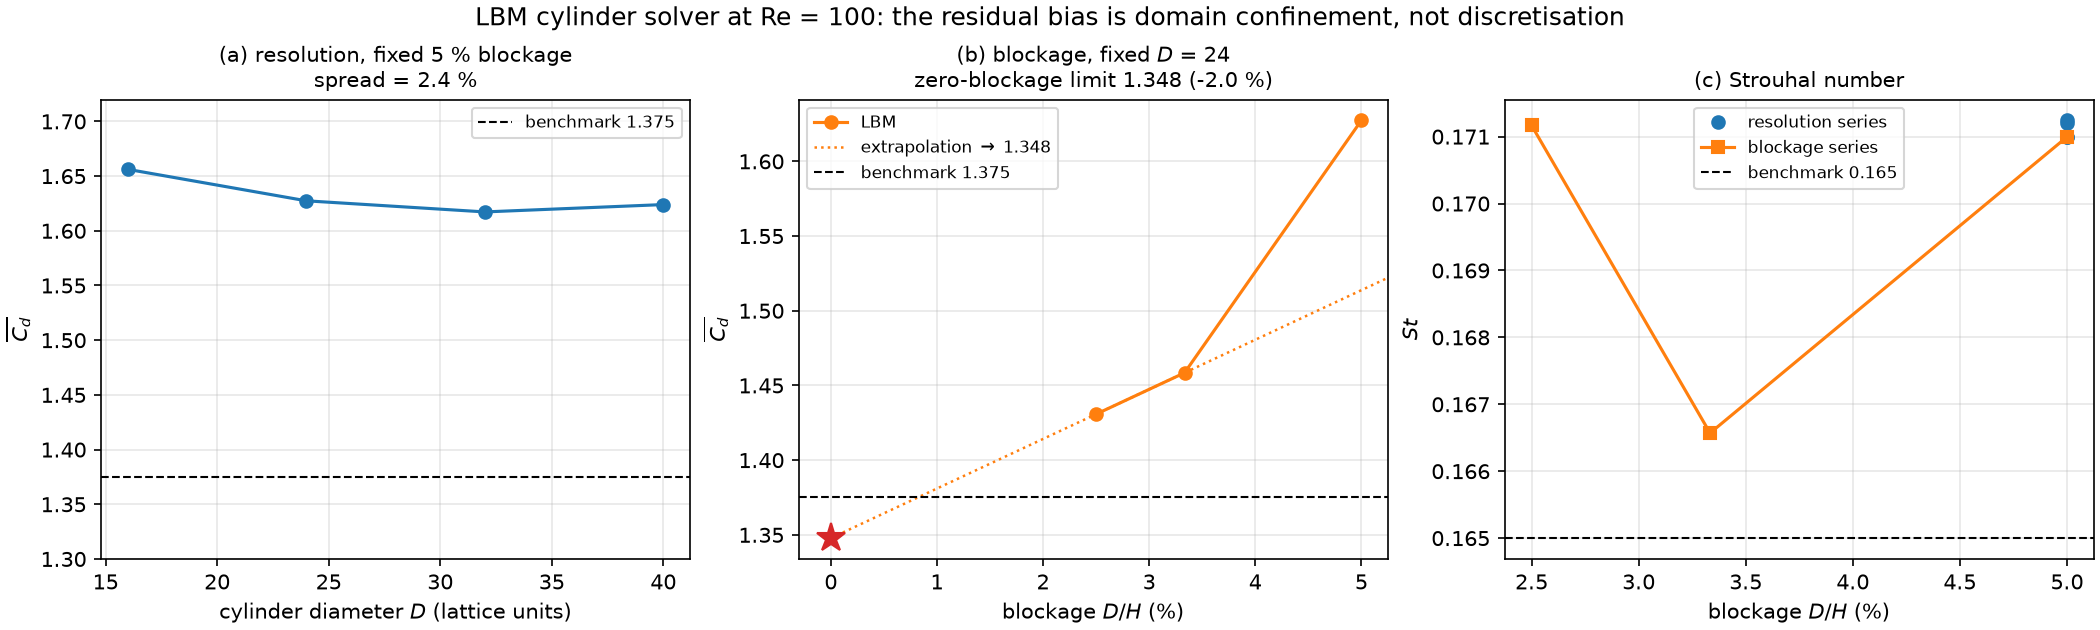
\includegraphics[width=0.92\textwidth]{convergence.png}
\caption{Solver validation: resolution series, blockage series, and the
extrapolation to zero blockage.}
\label{fig:convergence}
\end{figure}

\begin{figure}[h]
\centering
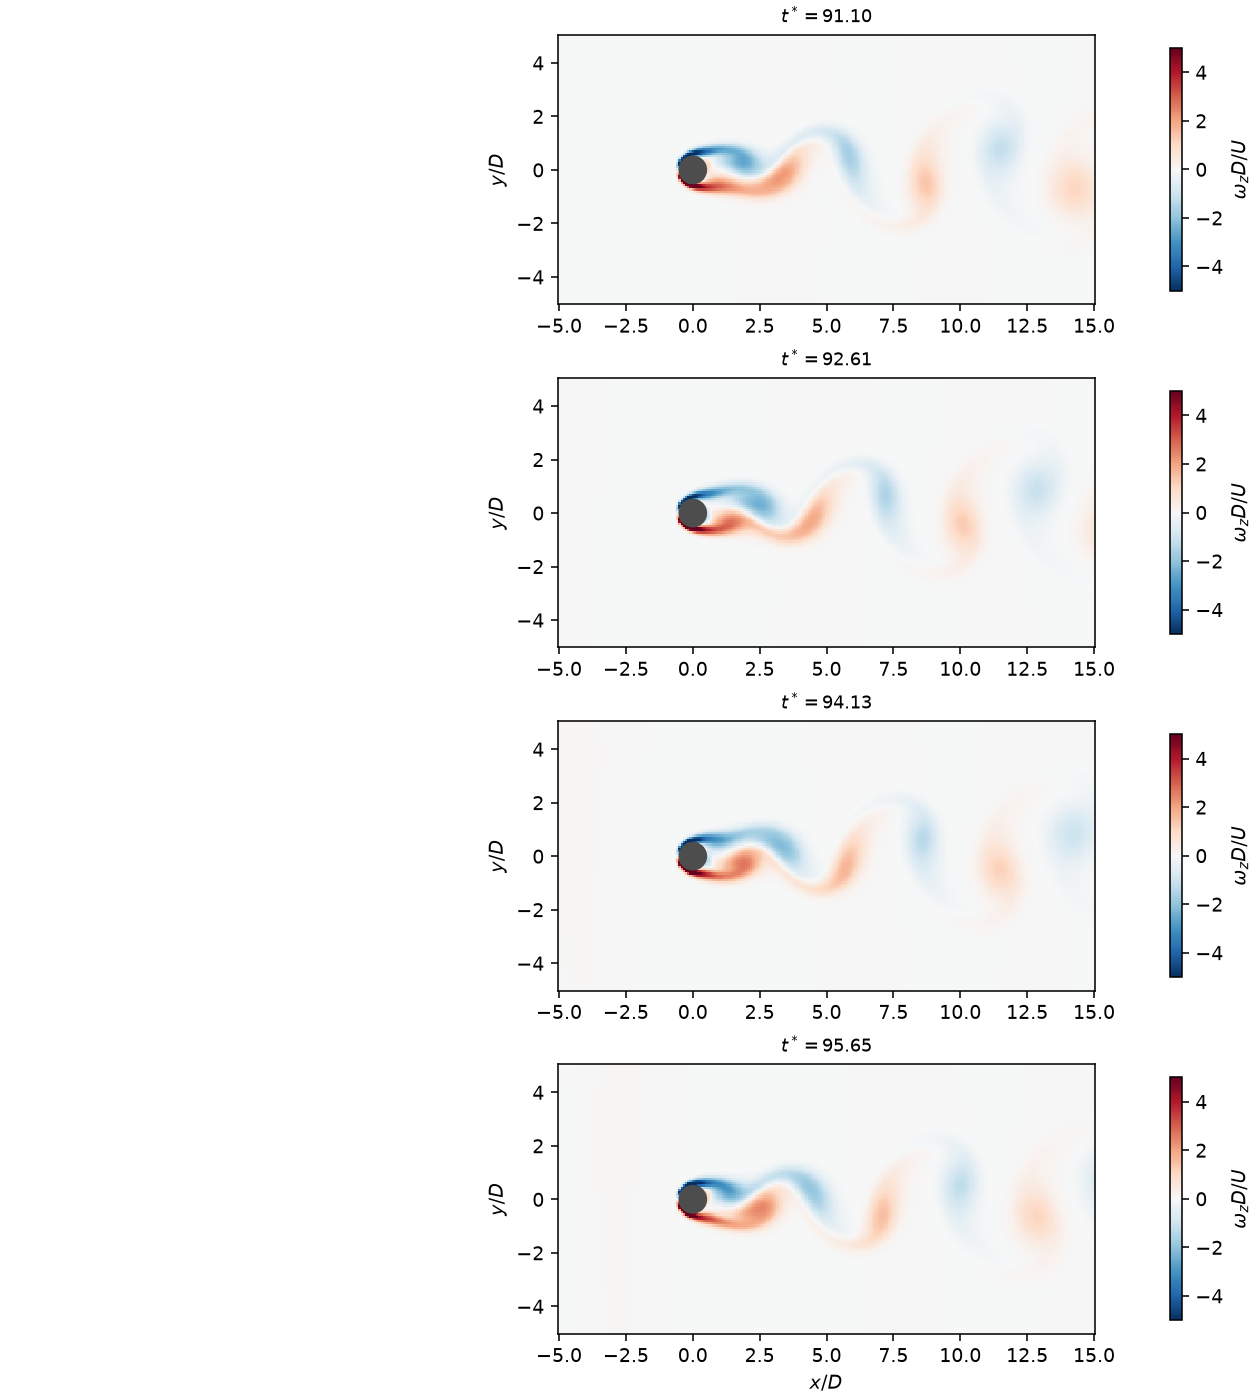
\includegraphics[width=0.92\textwidth]{re100_v4_vorticity.png}
\caption{The reference K\'arm\'an street over one shedding period.}
\label{fig:vorticity}
\end{figure}

\paragraph{A methodological note.} An early estimate of $\St$ taken from an FFT
peak gave a $+0.3\%$ agreement that was pure luck: with $\sim$12 recorded
periods the FFT bin width (0.014) exceeds the discrepancy being measured. All
$\St$ values reported here come from a zero-crossing estimator, which resolves
the period to a fraction of a time step; the honest error is $-2.3\%$.

\section{An unsteady Navier--Stokes operator}
\label{sec:operator}

\texttt{underPINN} ships only a steady incompressible residual, which cannot
represent shedding at all. This project supplies the unsteady operator
(\texttt{src/pinn/ns2d\_unsteady.py}), conforming to the framework's
\texttt{BasePDE} contract so it composes with the existing solvers, samplers
and networks. Non-dimensionalised on $D$ and $U$,
\begin{align}
u_x + v_y &= 0, \\
u_t + u u_x + v u_y + p_x - \tfrac{1}{\Rey}(u_{xx} + u_{yy}) &= 0, \\
v_t + u v_x + v v_y + p_y - \tfrac{1}{\Rey}(v_{xx} + v_{yy}) &= 0,
\end{align}
with the network mapping $(x,y,t) \mapsto (u,v,p)$.

Two derivative backends are implemented: a literal \texttt{jax.hessian}
reference, and a forward-over-forward JVP path computing only the six
derivative groups the residual needs, where a full Hessian would compute 27.

\begin{table}[h]
\centering
\caption{Verification of the unsteady operator. All three checks pass at
machine precision.}
\begin{tabular}{lc}
\toprule
check & result \\
\midrule
annihilates the Taylor--Green vortex (an exact NS solution) & $1.6\times 10^{-16}$ \\
fast JVP backend versus literal Hessian & $2.8\times 10^{-17}$ \\
steady limit versus \texttt{underPINN}'s own \texttt{NavierStokesPDE} & $5.6\times 10^{-17}$ \\
speed-up of the fast backend & $2.5\times$ \\
\bottomrule
\end{tabular}
\end{table}

The third check is the important one: it shows the new operator agrees with the
framework's existing physics, rather than being a parallel implementation that
merely looks correct.

\section{Reproducing the collapse}
\label{sec:collapse}

A plain multilayer perceptron $[3, 128^{\times 6}, 3]$ is trained on physics,
boundary and initial conditions with \emph{no data}, over a single time window
of one shedding period, for $20\,000$ epochs.

\begin{table}[h]
\centering
\caption{The documented failure, reproduced. Two seeds.}
\begin{tabular}{lcc}
\toprule
quantity & seed 0 & seed 1 \\
\midrule
shedding retained & 9.8\% & 11.3\% \\
relative $L_2$ on $(u,v)$ & 0.184 & 0.183 \\
\bottomrule
\end{tabular}
\end{table}

\emph{Shedding retained} is this project's own metric: the ratio of
transverse-velocity r.m.s.\ at a fixed wake probe between the PINN and the LBM
reference. Near 0\% means collapse to steady flow;
100\% means the wake amplitude matches.

The wake keeps about a tenth of the reference amplitude --- the PINN is
effectively solving the steady problem. Quadrupling the budget to $80\,000$
epochs moves this only to 21.9\%, so the collapse is not an
artefact of under-training.

\section{Defeating the collapse}
\label{sec:ablation}

Three mechanisms are implemented as switches on one trainer, so that the
ablation is controlled --- every configuration shares the sampler, the
optimiser, the schedule and the evaluation.

\begin{table}[h]
\centering
\caption{The ablation matrix: what each configuration attacks.}
\begin{tabular}{lll}
\toprule
configuration & mechanism & obstacle attacked \\
\midrule
\texttt{baseline}   & --- & (control) \\
\texttt{fourier}    & random Fourier features & spectral bias \\
\texttt{decompose}  & Reynolds decomposition $u = u_0 + u'$ & conditioning, dynamic range \\
\texttt{march}      & causal time-marching & weak initial condition, causality \\
\texttt{all}        & all three & --- \\
\texttt{all+data}   & plus $4\,000$ supervised points per window & --- \\
\bottomrule
\end{tabular}
\end{table}

Two implementation points matter. First, the Reynolds decomposition requires a
\emph{differentiable} mean field, because the momentum residual contains
$\nabla u_0$ and $\nabla^2 u_0$; bilinear interpolation of a grid gives
piecewise-constant first derivatives and identically zero second derivatives.
The mean is therefore fitted by a separate frozen network (relative
$L_2 = 1.1\times 10^{-3}$). Second, that mean is obtained by \emph{regression on the
measured mean}, not by a steady PINN solve, because the time mean of a shedding
flow does not satisfy the steady equations --- it carries the divergence of the
Reynolds stresses.

\subsection{Result}

\begin{table}[h]
\centering
\caption{Full-budget ablation at $\Rey = 100$: $20\,000$ epochs per window,
two seeds, seed means. \emph{Time-marching alone is sufficient, data-free.}}
\begin{tabular}{lcc}
\toprule
configuration & shedding retained & relative $L_2$ \\
\midrule
\texttt{baseline}  & 10.6\% & 0.183 \\
\texttt{fourier}   & 9.7\%  & 0.167 \\
\texttt{decompose} & 7.0\%  & 0.110 \\
\texttt{march}     & \textbf{89.2\%} & 0.078 \\
\texttt{all}       & \textbf{90.2\%} & 0.047 \\
\texttt{all+data}  & 100.0\% & \textbf{0.015} \\
\bottomrule
\end{tabular}
\end{table}

\begin{figure}[h]
\centering
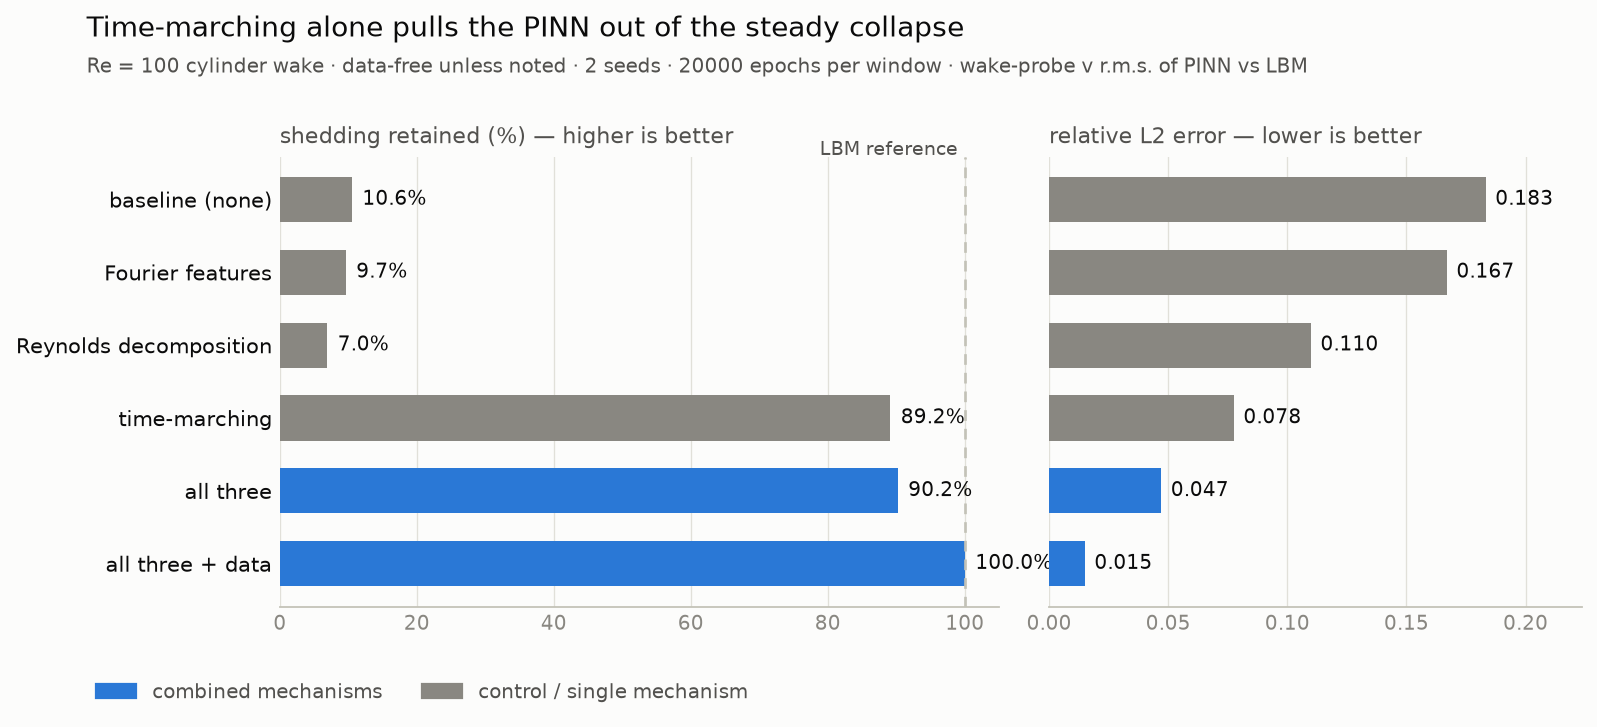
\includegraphics[width=\textwidth]{ablation.png}
\caption{The ablation. Neither Fourier features nor the Reynolds decomposition
escapes the collapse; causal time-marching does.}
\label{fig:ablation}
\end{figure}

Neither spectral bias nor conditioning was the binding constraint. Both
mechanisms reduce the field error --- the decomposition notably, from 0.183 to
0.110 --- while leaving the wake collapsed. What restores shedding is enforcing
causality: solving a short window, then using its end state as the initial
condition for the next, which strengthens the initial condition relative to the
bulk residual and forbids information from flowing backwards in time.

\subsection{The equal-budget control}

A marched run of four windows takes four times the optimiser steps of a
single-window run, so the comparison above is confounded by compute. Re-running
the single-window configurations at $80\,000$ epochs --- the same total ---
settles it:

\begin{table}[h]
\centering
\caption{Equal-budget control. Both improve; neither approaches
89\%. \emph{The gain is causality, not compute.}}
\begin{tabular}{lccc}
\toprule
configuration & $20\,000$ ep, 1 window & $80\,000$ ep, 1 window & $4\times 20\,000$ ep, 4 windows \\
\midrule
\texttt{baseline}  & 10.6\% & 21.9\% & --- \\
\texttt{decompose} & 7.0\%  & 23.8\% & --- \\
\texttt{march}     & ---                 & ---                 & \textbf{89.2\%} \\
\bottomrule
\end{tabular}
\end{table}

This control is essential to the claim and should be quoted with it; without
it, ``time-marching wins'' is indistinguishable from ``time-marching trains
longer''.

\subsection{Hyperparameters, and one that mattered only in combination}

\begin{table}[h]
\centering
\caption{Knobs, two seeds each.}
\begin{tabular}{llcc}
\toprule
change & applied to & shedding retained & relative $L_2$ \\
\midrule
$\sigma = 8$ (from 2) & \texttt{all}     & 90.2\% $\rightarrow$ \textbf{97.6\%} & 0.047 $\rightarrow$ \textbf{0.042} \\
$\sigma = 8$          & \texttt{fourier} & 9.7\% $\rightarrow$ 11.9\% & 0.167 $\rightarrow$ 0.147 \\
$w_{ic} = 100$ (from 10) & \texttt{all}  & 90.2\% $\rightarrow$ 89.8\% & no change \\
\bottomrule
\end{tabular}
\end{table}

The Fourier bandwidth $\sigma$ is worth several points \emph{on top of} the
mechanism that works, and nothing at all without it. The initial-condition
weight, by contrast, changes nothing once marching supplies the causal chain
--- consistent with the interpretation that marching works by strengthening
the initial condition, making further weighting redundant.

\subsection{How much supervision is actually needed}

\begin{table}[h]
\centering
\caption{Supervised points per window, two seeds, seed means.}
\begin{tabular}{lcc}
\toprule
data points per window & shedding retained & relative $L_2$ \\
\midrule
0    & 90.2\% & 0.047 \\
100  & 96.2\% & 0.030 \\
500  & 97.6\% & 0.021 \\
2000 & 99.5\% & 0.016 \\
4000 & 100.0\% & 0.015 \\
\bottomrule
\end{tabular}
\end{table}

Shedding saturates by 100 points per window; everything beyond that buys
accuracy only. \emph{The physics buys the dynamics; the data buys the last
factor of three in error.}

\section{How accurately does it shed?}
\label{sec:accuracy}

Shedding retained is an amplitude ratio: it answers ``is there a wake'', which
is the right question for the collapse and the wrong one for prediction
accuracy. A network could hold the right amplitude at the wrong frequency, or
drift out of phase within the window, and the ablation table would not notice.
The best data-free configuration was therefore compared against the reference
probe signal directly.

\begin{table}[h]
\centering
\caption{Prediction accuracy of the best data-free configuration (\texttt{all},
$\sigma = 8$) at $\Rey = 100$, over one shedding period and over five.}
\begin{tabular}{lccc}
\toprule
quantity & 1 period (4 windows) & 5 periods (20 windows) & reference \\
\midrule
shedding frequency $\St$ & 0.1565 ($-0.9\%$) & \textbf{0.1622 ($+0.1\%$)} & 0.1621 (LBM) \\
wake amplitude           & 96.5\% & 94.8\% & LBM probe r.m.s. \\
phase lag                & $+2.9^\circ$ & $+2.4^\circ$ & --- \\
phase drift across span  & $-0.000$ periods & $-0.005$ periods & --- \\
velocity-field error     & 0.043 & \textbf{0.036} & relative $L_2$ \\
zero crossings available & 2 & 10 & 12+ for the LBM's own $\St$ \\
\bottomrule
\end{tabular}
\end{table}

Extending the run from four windows to twenty --- from one shedding period to
five --- \emph{improves} every quantity that matters. The frequency error falls
to $+0.1\%$ on ten zero crossings rather than two, the field error drops from
0.043 to 0.036, and the phase drifts by $0.005$ of a period (about $2^\circ$)
across the entire five-period span. The marching chain therefore does not
accumulate error in any visible way over the horizon tested: the wake stays
locked to the reference in both frequency and phase, and only the amplitude
gives up a little (96.5\% to 94.8\%).

\begin{figure}[h]
\centering
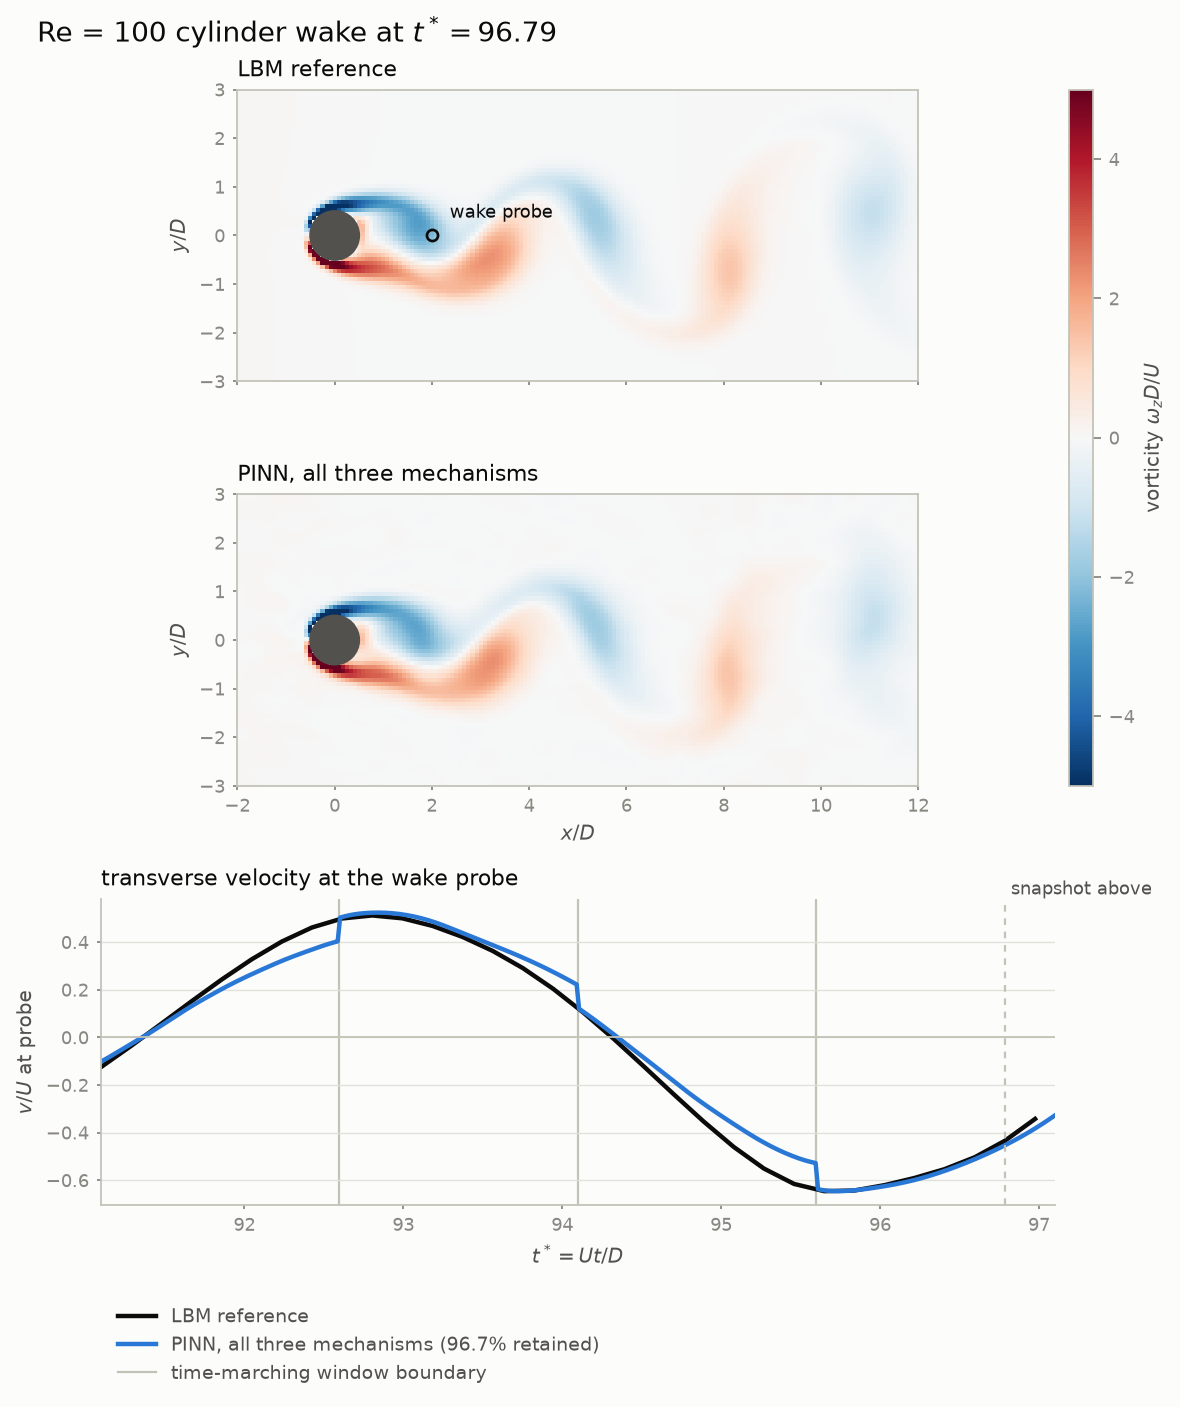
\includegraphics[width=0.85\textwidth]{fields_best.png}
\caption{The data-free PINN against the reference. A K\'arm\'an street from a
network that never saw data. The small steps in the probe trace are the
time-marching window handoffs.}
\label{fig:fields}
\end{figure}

\paragraph{Caveat.} Ten zero crossings is enough to state $\St$ to about a
percent, but it is still a shorter record than the LBM's own validation
(${\sim}12$ periods of a signal that is not itself being predicted). The
frequency agreement to $+0.1\%$ should be read as ``within the resolution of
this measurement'', not as a claim of three-digit accuracy.

\paragraph{Visible artefact.} The probe trace shows small discontinuities at
window handoffs, where each window starts from the previous one's end state
rather than continuing it smoothly. This is the cost of the mechanism that
makes the wake survive, and is reported rather than smoothed away.

\section{Physics in a neural operator}
\label{sec:fno}

The reference paper's FNO is purely data-driven. This section reproduces its
recipe and then asks whether physics improves it.

\paragraph{Reproduction.} \texttt{underPINN}'s \texttt{FNO2D}, trained after
Renn et al.: Reynolds-decompose first, map two consecutive frames to the next,
apply recursively for ten steps during training with the loss summed over every
step; width 80, 24 modes, Adam at $1\times 10^{-3}$, 200 epochs, batch 16.

\paragraph{Contribution.} A physics residual is added to that loss. The network
predicts $(u,v)$ only, so any residual containing $\nabla p$ is unusable;
taking the curl of the momentum equations removes the pressure and leaves
vorticity transport,
\begin{equation}
\omega_t + u\,\omega_x + v\,\omega_y - \tfrac{1}{\Rey}\nabla^2 \omega = 0,
\qquad \omega = v_x - u_y ,
\end{equation}
evaluated by finite differences on the grid. Continuity is available
separately as the cheaper variant. Both residuals are normalised by the
residual the LBM data \emph{itself} leaves --- the data is weakly compressible
and second-order accurate, so driving a prediction below that floor would be
fitting discretisation error, not physics.

\begin{table}[h]
\centering
\caption{Rollout error (relative $L_2$ on $(u,v)$, held-out initial
conditions, two seeds). The trained horizon is ten steps.}
\begin{tabular}{lcccc}
\toprule
forecast steps & 10 (trained) & 20 & 30 & 50 \\
in shedding periods & 0.31 & 0.61 & 0.92 & 1.53 \\
\midrule
\texttt{data} (paper recipe)        & 0.093 & 0.183 & \textbf{0.296} & \textbf{0.365} \\
\texttt{physics} (continuity + vorticity) & \textbf{0.074} & \textbf{0.132} & 0.307 & 0.772 \\
\texttt{physics\_div} (continuity only)   & 0.075 & 0.140 & 0.312 & 0.764 \\
\bottomrule
\end{tabular}
\end{table}

\begin{figure}[h]
\centering
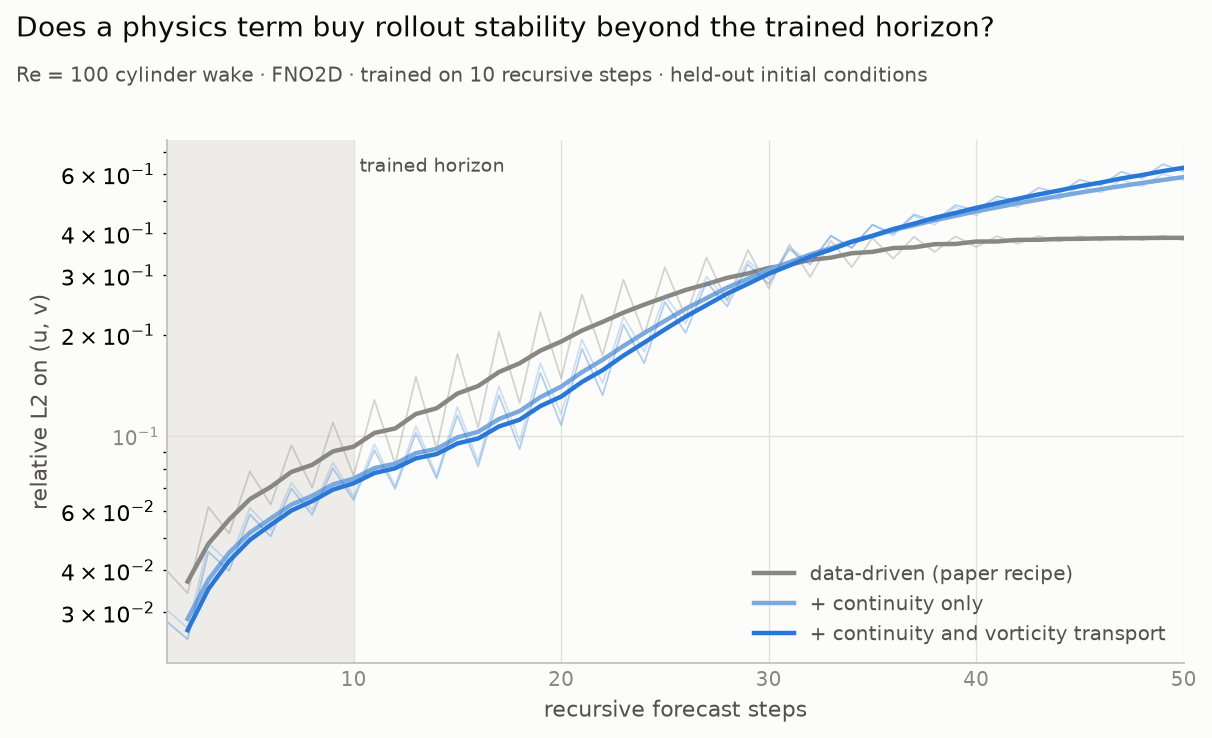
\includegraphics[width=\textwidth]{fno.png}
\caption{Forecast error against horizon. Bold lines are pairwise means over
adjacent steps; faint lines are raw (see the parity note). The curves cross at
approximately one shedding period.}
\label{fig:fno}
\end{figure}

\paragraph{Result.} Physics lowers forecast error by 20\% at the
trained horizon and 28\% at twice it, then \emph{crosses over} at
step 27--32 across seeds and variants, which is 0.8--1.0 shedding
periods. Continuity alone buys nearly all of the benefit, so the effect is not
specific to the vorticity term --- useful, since continuity is the cheaper
residual by far.

\paragraph{Why the late-horizon ordering is not reported as a result.} By 50
steps both variants have failed in the sense that matters: the error on the
fluctuation exceeds unity, meaning that predicting zero fluctuation would beat
either rollout. The data-driven curve flattens because it decays towards the
mean flow --- the safest wrong answer --- while the physics-constrained
rollouts keep injecting fluctuation energy and overshoot. Across seeds the
physics variant reads 0.63 and 0.92 at 50 steps, so the gap is not
reproducible. The defensible statement is that \emph{physics extends the useful
forecast horizon, and neither model is usable beyond one shedding period}.

\paragraph{A parity artefact worth naming.} Rollout error alternates between
even and odd steps by 30--45\% in \emph{every} variant,
physics or not: a period-2 mode of the two-frame autoregressive map. A single
step's error can therefore read 30\% better or worse purely by
which parity it lands on, so all numbers above are pairwise means of adjacent
steps, and the figure keeps the raw curve visible.

\paragraph{Comparison with the reference paper.} At the trained horizon the
data-driven variant reaches $\epsilon = 0.093$ against the paper's
$\epsilon < 0.1$. \emph{This is not an improvement on their work.} Our data is
clean, periodic, two-dimensional LBM output at $\Rey = 100$; theirs is noisy
experimental PIV at $\Rey = 240$--$3060$ with genuine three-dimensionality. The
only claim supported is that the reproduction works.

\FloatBarrier
\section{Conclusions}

\begin{enumerate}
  \item The documented collapse reproduces on validated ground truth: a
        data-free PINN retains 10.6\% of the wake, and quadrupling
        the training budget does not fix it.
  \item \textbf{Causal time-marching alone restores shedding, data-free}
        (89.2\% retained), and an equal-budget control attributes
        the gain to causality rather than to compute. Fourier features and the
        Reynolds decomposition do not escape the collapse on their own, but
        improve accuracy substantially once marching is in place, taking the
        field error from 0.078 to 0.042.
  \item The best data-free configuration predicts the shedding frequency to
        0.9\%, the amplitude to 96.5\% and the phase
        to $3^\circ$, over one shedding period, with a velocity-field error of
        4.3\%.
  \item Supervision is needed in far smaller quantity than expected: 100 points
        per window restores 96\% of the shedding, and further data
        buys accuracy only.
  \item Adding a pressure-free physics residual to a data-driven FNO lowers
        forecast error by 20--28\% within one shedding
        period, with continuity alone responsible for nearly all of it. Beyond
        one period both variants fail.
\end{enumerate}

\section{Limitations and ongoing work}
\label{sec:ongoing}

\begin{itemize}
  \item \textbf{One Reynolds number.} Every result above is at $\Rey = 100$. A
        sweep over $\Rey = 60, 80, 120, 150, 180$ is running, repeating the
        \texttt{baseline}-versus-\texttt{all} comparison at each, with the
        marching window scaled to each dataset's measured shedding period so
        the configurations stay comparable. The upper limit is set by the
        three-dimensional transition near $\Rey \approx 190$.
  \item \textbf{Five shedding periods of PINN evaluation.}
        Section~\ref{sec:accuracy} covers five periods, over which the accuracy
        improves rather than decays. Behaviour over tens of periods, where a
        marching chain might accumulate phase error, is untested --- and the
        cost grows linearly with the horizon, one window per quarter period.
  \item \textbf{$\Cl$ r.m.s.\ is not converged} across configurations
        (0.18--0.54 against a benchmark of $\sim$0.23) and is deliberately not
        quoted as a validation metric.
  \item \textbf{The resolution series was run at 5\% blockage},
        where blockage masks resolution. The blockage series is sound; a clean
        resolution answer would require repeating it at $H = 40D$.
\end{itemize}

\paragraph{A note on method.} Estimates for each phase were recorded
\emph{before} running it. Three were wrong in ways that changed conclusions:
the collapse was expected to need all three mechanisms (it needs one); the
Fourier bandwidth was expected to be the quick win (it does nothing alone); and
the FNO physics term was expected to help only beyond the trained horizon (it
helps within it and hurts beyond). An earlier CPU sweep at a fifth of the
budget supported the first of those wrong conclusions --- \emph{an under-trained
ablation produces the wrong qualitative answer, not merely a noisier one.}

\begin{thebibliography}{9}
\bibitem{renn2023}
P.~J. Renn, C.~Wang, S.~Lale, Z.~Li, A.~Anandkumar and M.~Gharib,
\emph{Forecasting subcritical cylinder wakes with Fourier Neural Operators},
arXiv:2301.08290, 2023.

\bibitem{pinnfail}
\emph{Can physics-informed neural networks beat the finite element method?}
--- and related analyses of PINN failure modes in unsteady flow,
arXiv:2306.00230, 2023.

\bibitem{underpinn}
Aeroscience Computations and Analysis Lab, \texttt{underPINN}: a JAX framework
for physics-informed neural networks.
\end{thebibliography}

\end{document}
